% !TEX root = Bachelorarbeit Synthetische Daten.tex
\chapter{Methodisches Vorgehen}

In diesem Kapitel wird das methodische Vorgehen der Arbeit beschrieben. Als Basis für die Untersuchung der Forschungsfragen wird zunächst der MVIP-Datensatz vorgestellt, auf dem die Experimente durchgeführt werden. Anschließend wird die Implementierung der Modelle DA-Fusion und Supervised Contrastive Learning erläutert, die für die synthetische Datengenerierung und die Klassifikationsaufgabe verwendet werden. Es wird auch auf die Anpassungen eingegangen, die vorgenommen werden mussten, um den eigenen Ansatz zu testen. Danach wird die Herangehensweise zur Generierung synthetischer Daten mit DA-Fusion und die Trainings- und Testdurchläufe mit Supervised Contrastive Learning definiert. Abschließend werden die Evaluationsmethoden und Metriken vorgestellt, die zur Auswertung der Experimente verwendet werden.

\section{MVIP-Datensatz} \label{sec:dataset}

Grundlage der Forschungsarbeit ist der im Rahmen des EIBA-Projekts entstandene MVIP-Datensatz \parencite{Koch2023mvip}, wobei MVIP für \textit{Multi-View Industrial Parts} steht. Er enthält 308 Klassen, welche wiederum in 18 verschiedene Oberklassen (Super Classes) eingeteilt sind. Insgesamt gibt es etwa 71.276 Sets an Bildern, die jeweils RGB- und Tiefendaten, sowie Segmentierungsmasken enthalten.

Die Bilddaten stammen aus Intel RealSense D435 und D415 Tiefenkameras, die die Objekte gleichzeitig aus verschiedenen Perspektiven aufnehmen. Darüber hinaus gibt es auch Metadaten, etwa zum Gewicht des Objekts, oder Beschreibungen in natürlicher Sprache durch verschiedene Stichwörter ("StarterMotor", "Used", "Rusty", usw.).

% Beispielbilder, -masken, -metadaten
\begin{figure}[]
	\centering
	%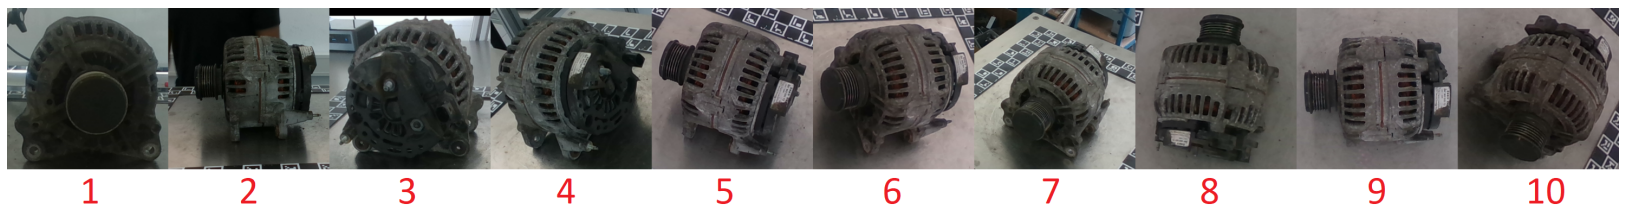
\includegraphics[width=\textwidth]{figure_mvip_ex_cropped_1.png}
	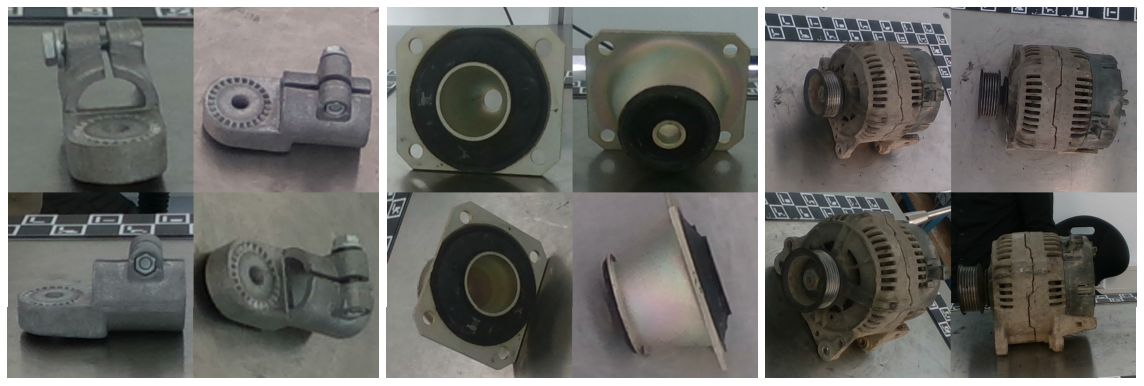
\includegraphics[width=\textwidth]{figure_mvip_ex_cropped_2.png}
	\caption{Beispielbilder aus dem MVIP-Datensatz \parencite{Koch2023mvip},\\
	die auf die Region of Interest (ROI) zugeschnitten wurden.}
	\label{fig:mvip-examples}
\end{figure}

\subsection{Teildatensatz} \label{sec:subdataset}

% Wahl eines Teildatensatzes mit 20 "CarComponent" Klassen
Da für die Experimente relativ viele Trainings- und Testdurchläufe vorgesehen waren, war es notwendig, einen Teildatensatz auszuwählen, um die Rechenzeit zu reduzieren.

Konkret wurden zufällig 20 Klassen aus der Oberklasse "CarComponent" ausgewählt. Für die Experimente wurden nur die RGB-Bilddaten verwendet, wobei die Segmentierungsmasken im Pre-Processing zum Einsatz kommen (siehe Abschnitt \ref{sec:preprocessing}).

Insgesamt enthält der Teildatensatz ... Bilder. In Tabelle \ref{tab:subdataset} sind die Klassen und die Anzahl der Bilder pro Klasse aufgeführt.

\begin{table}[h]
	%\centering
	\caption{Auswahl der 20 Klassen aus der Oberklasse "CarComponent"\\
	für den Teildatensatz.}
	\begin{tabular}{|l|l|c|}
		\hline
		\textbf{Klasse} & \textbf{Beschreibungen} & \textbf{Anzahl Bilder} \\
		\hline
		... & ... & ... \\
		\hline
	\end{tabular}
	\label{tab:subdataset}
\end{table}

\subsection{Vorverarbeitung} \label{sec:preprocessing}

% Verwendung der Objektmasken, um die Bilder zu croppen
	% Bounding Box
	% Quadratischer Output
	% Weniger Aufmerksamkeit auf gleichbleibenden Hintergrund
Die Vorverarbeitung der Bilder unterscheidet sich nur leicht zwischen den beiden Modellen DA-Fusion und Supervised Contrastive Learning. In beiden Fällen werden die Bilder auf die Region of Interest (ROI) zugeschnitten, um den Fokus auf die Objekte zu legen und den Hintergrund zu minimieren. Dazu werden die Segmentierungsmasken verwendet, um die Bounding Box der Objekte zu bestimmen und die Bilder entsprechend zuzuschneiden. Die Ausgabe ist ein quadratisches Bild, das die Objekte in der Mitte enthält.

% Verschiedene "klassische" Augmentationen
	% Rotation
	% ColorJitter
	% Normalisierung
Zusätzlich werden verschiedene "klassische" Augmentationen angewendet, um die Daten zu erweitern und die Modelle robuster zu machen. Dazu gehören z.B. Rotation, ColorJitter und Normalisierung. Die Parameter für die Augmentationen wurden eher konservativ gewählt, damit die feinen Unterschiede zwischen den Klassen nicht verwischt werden.

\section{Implementierung} \label{sec:implementation}

% Einleitung, Arbeitsumgebung, Rechner-Zugang, etc.
Zur Vorbereitung und Durchführung der Experimente wurde seitens des Fraunhofer-IPK ein Zugang zu einem leistungsstarken Rechner bereitgestellt, der über zwei NVIDIA-Grafikkarten mit CUDA-Unterstützung verfügt.

Dabei konnte sich größtenteils auf die Implementierung von DA-Fusion und Supervised Contrastive Learning aus den Quellen \parencite{Trabucco2024dafusiongithub} und \parencite{Tian2023supcongithub} gestützt werden. Dennoch mussten einige Anpassungen vorgenommen werden, die nun erläutert werden.

\subsection{DA-Fusion} \label{sec:impl-da-fusion}

% Klasse zum Laden des MVIP-Teildatensatzes
	% Masken-cropping
	% Masken für Augmentation

% Workflow-Anpassungen für Input/Output

In ...'s Implementierung von DA-Fusion wird zunächst mit Textual Inversion ein vortrainiertes Stable Diffusion-Modell fine-tuned, indem ein neuer Token für jede Klasse im Datensatz erlernt wird. Um anschließend die Augmentationen zu generieren, werden die Bilder des Datensatzes genommen, Rauschen hinzugefügt und unter Konditionierung auf den entsprechenden Token wiederhergestellt. Je nachdem, wie viel Rauschen hinzugefügt wurde, entstehen so mehr oder weniger stark veränderte Bilder, die als synthetische Daten verwendet werden können.

...

Die Implementierung von DA-Fusion kann weitgehend unverändert angewendet werden, um synthetische Daten für den MVIP-Teildatensatz zu generieren. Es muss lediglich eine eigene Klasse für den Datensatz erstellt werden, die die Bilder und Masken aus dem MVIP-Datensatz lädt und die Token für die Klassen bereitstellt. ...

\subsection{Supervised Contrastive Learning} \label{sec:impl-supcon}

% Klasse zum Laden des MVIP-Teildatensatzes und der Augmentationen

% Workflow-Anpassungen für Input/Output (wie DA-Fusion)

% Parameter für Konfiguration der Verwendung der Augmentationen

% Integration von OOD-Augmentationen im Contrastive Learning

% Metriken für Evaluation
	% Accuracy
	% ID- und OOD-Confidence

...'s Implementierung von Supervised Contrastive Learning beinhaltet drei Trainings-Skripte; eines für das Pre-Training der latenten Repräsentationen unter Verwendung der Supervised Contrastive Loss-Funktion, eines für die lineare Klassifikation der Repräsentationen und eines zum Training eines klassischen Klassifikator-Modells mit Cross Entropy Loss (zum Vergleich).

...

Auch hier muss eine eigene Klasse für den MVIP-Teildatensatz erstellt werden, die die Bilder und Masken lädt und die synthetischen Daten von DA-Fusion bereitstellt. Die Klasse muss nun auch Parameter bereitstellen, die die Verwendung der synthetischen Daten steuern, z.B. ob keine Augmentationen, ausschließlich positiv-Beispiele oder auch negativ-Beispiele verwendet werden sollen. ...

...

\section{Synthetische Datengenerierung mit DA-Fusion} \label{sec:synt-gen-da-fusion}

% ID-Augmentationen, OOD-Augmentationen
% Trial and Error, um Parameter zu bestimmen, Validierung ist schwierig
...

\section{Trainings- und Testdurchläufe mit Supervised Contrastive Learning} \label{sec:train-test-supcon}

% Drei Versuche; jeweils Contrastive Pre-Training & Lineare Klassifikation
Die Trainings- und Testdurchläufe mit Supervised Contrastive Learning sind in drei Versuchsreihen unterteilt. In jedem Versuch wird zunächst das Pre-Training der latenten Repräsentationen durchgeführt, gefolgt von der linearen Klassifikation der Repräsentationen. Die Versuchsreihen unterscheiden sich in der Verwendung der synthetischen Augmentationen:

\begin{enumerate}[font=\bfseries]
	\item \textbf{Versuch}: Nur reale Daten werden verwendet, sowohl für das Pre-Training als auch für das Training des Klassifikators.
	\item \textbf{Versuch}: Neben den realen Daten werden auch ID-Augmentationen verwendet, sowohl für das Pre-Training als auch für das Training des Klassifikators.
	\item \textbf{Versuch}: Wie Versuch 2, aber im Pre-Training werden zusätzlich Near OOD-Augmentationen als harte negativ-Beispiele verwendet, wie in Abschnitt \ref{sec:da-fusion-supcon} beschrieben.
\end{enumerate}

% Hyperparameter
Für das Pre-Training wurde eine Batch Size von 16, eine Lernrate von 0.001 mit Kosinus-Annealing und einer Dauer von 110 Epochen verwendet. Die Bilddaten wurden im Rahmen der Augmentation auf eine Größe von 224x224 Pixeln zugeschnitten und normalisiert. Bei der linearen Klassifikation sind die Hyperparameter identisch, jedoch mit einer Dauer von 25 Epochen.

% Evaluierung auf Testdaten
Nach den Trainingsdurchläufen werden die Modelle auf den (echten) Testdaten evaluiert.

\section{Evaluationsmethoden und Metriken} \label{sec:evaluation}

Die Qualität der synthetischen Daten, die mit DA-Fusion generiert wurden, werden durch einfache visuelle Inspektion selbst überprüft. Bei den ID-Augmentationen wird darauf geachtet, dass die Objekte in den Bildern in ihrer Form möglichst unverändert bleiben, während die Farben und Texturen variieren können und sollen. Bei den OOD-Augmentationen wird darauf geachtet, dass die Objekte stark genug verändert werden, um nicht mehr als Beispiele für die ID-Klassen erkannt zu werden, während sie gleichzeitig noch genug Ähnlichkeit aufweisen, um herausfordernde negative Beispiele zu sein.

% Menschliche Evaluierung der Augmentationen selbst
% Accuracy, ID- und OOD-Confidence des SCL Klassifikators
Die Ergebnisse der drei Versuchsreihen werden ausgewertet, indem folgende Metriken beim Test der linearen Klassifikation auf den Testdaten gemessen werden:

\begin{itemize}
	\item \textbf{Accuracy}: Der Anteil der korrekt klassifizierten Beispiele.
	\item \textbf{ID-Confidence}: Die durchschnittliche Konfidenz des Klassifikators auf den ID-Daten.
	\item \textbf{OOD-Confidence}: Die durchschnittliche Konfidenz des Klassifikators auf den OOD-Daten.
\end{itemize}